

\documentclass{article}


\usepackage[a4paper, margin=3.0cm]{geometry}


\usepackage{graphicx}
\usepackage{float}
\usepackage{hyperref}



\title{Investigating properties of displaced jets stemming from long-lived gluinos (DRAFT)}
\author{Me, Matthias, Vilius?}
\date{\today}

\begin{document}

\maketitle

\begin{abstract}
Abstract
\end{abstract}

\section*{Introduction}
The standard model of particle physics (SM), despite being a triumph of modern physics with its predictions of new particles such as the W and Z bosons, has known holes where it does not predict what is observed. One of the leading beyond-the-standard-model (BSSM) theories is supersymmetry (SUSY), however experimental evidence of this has yet to be observed. 


Dark matter is another mystery, making up the majority of matter in the universe yet currently we can only speculate about its nature. Given that is is likely massive and weakly-interacting with SM particles, supersymmetric particles are a possible candidate. Some extensions of the SM also predict particles with long lifetimes (cite something!), which would lead to unique signatures in the detectors, since the SUSY particle would not interact but some of its decay products might, leading to displaced vertex decays. These are particularly interesting since nothing in the SM would give a displaced vertex, meaning that the background is very low.

A simple model of DM production at the LHC has it decaying into two gluinos, which are the long lived particles (LLPs) in this scenario. These gluinos then propagate a certain distance through the detector before decaying into four jets and two DM particles, taken as the lightest supersymmetric particle (LSP), neutralinos, denoted by $\chi_{0}$ in Figure \ref{feyn}. The expected signature is therefore four displaced jets and missing transverse energy. 

\begin{figure}[H]
\centering
\includegraphics[width=8cm]{glufeyn.png}
\caption{Feynman diagram of the expected interaction. }
	\label{feyn}
\end{figure}


However, gluino radiation from the colliding protons introduces initial state radiation (ISR), which increases the number of jets per event. Nonetheless, displaced vertices remain an interesting target for the high-luminosity run of the LHC.

This analysis investigates the properties of the detected jets from long-lived gluinos, in order to improve any future analyses of simulated or actual data. The two main unknowns are the mass of the gluino, and the lifetime of the gluino, so the dependence of (something) variables on both of these is investigated to (solidify) the shapes of the expected signature. The spacial distribution of jets is also explored along with the mean number of jets seen, in order to estimate the effect of the ISR jets on the sample. 

Then, the effect of the current JetId analysis tool on the data was investigated for the jets to determine whether it was useful in this particular scenario or whether it could be improved in some way. To aid with this, the best possible individual cut efficiencies were also calculated and compared.

Two methods of selecting the gluino jets were tested on the data using the invariant mass of the jets. First, the four jets with the two highest invariant masses were taken as the gluino jets, then the four jets with the two most similar invariant masses were used, since the gluinos would be expected to have similar masses. The dependence of the invariant mass on the LLP mass was also verified, and the mass asymmetry of the gluino jets investigated. From this, the resultant transverse momentum (pT) of the gluino system is found, as one would expect it to be non-zero due to the presence of the LSP particle. 
	
Finally, two cases for the LLP and LSP masses were compared. Since both their masses are unknown, it is instructional to consider both the compressed ($M_{LLP} \approx M_{LSP}$) and uncompressed ($M_{LLP} >> M_{LSP}$) cases, to determine how this distribution of masses affects the distributions of notable variables.  




\section*{Something about data (need more?)}
The monte carlo data used for the analysis contains a total number of 5483660 events. These events are grouped according to their $c_{\tau}$ value, ranging from 1$\mu$m to 100m, and contain decays of gluinos with masses ranging from 600 GeV/$c^{2}$ to 2400 GeV/$c^{2}$ and LSP masses ranging from 200 GeV/$c^{2}$ to 1400 GeV/$c^{2}$.

During the analysis, in general not all events were used for all plots due to investigating the effects of changing the masses or $c_{\tau}$. The number of events per lifetime is also not constant, so any comparisons of jet number presented in this note are normalised to jets per event for greater clarity.

\section*{Analysis results}
\subsection*{Variable dependence on gluino mass and $c_{\tau}$}
Initially, the pT of all the jets in each event was summed over to find the Ht, with a basic cut of 30 GeV/c and only jets that would be within the central part of the detector included. At fixed $c_{\tau}$, the distibution shows two main features, the the peak at higher gluino masses and the decaying shape for lower masses. The decay shape for lower masses does not seem to have strong dependence on the LLP mass, however at higher masses the peak position shifts to higher Ht the higher the gluino mass. 

Comparing the plots for different $c_{\tau}$, we see that the high-lifetime peaks start to become less distinct from the low-lifetime shape, until they finally merge with it. This drop off begins subtly at $c_{\tau}$ = 1m, and by $c_{\tau}$ = 10m and 100m has decreased substantially. This is likely a consequence of the ISR, since at low $c_{\tau}$, the gluinos decay well inside the detector, so all four jets are included in the Ht calculation, as well as the ISR jets. However, at larger $c_{\tau}$, the gluino is displaced closer to the edge of the detector, so one or more of its jets may be outside the detector and are therefore not detected. This means that the only jets included in the calculation are the ISR jets, so only their distinctive shape remains. Another implication of Figure \ref{htctau} is that Ht as a variable may be less useful as a single analysis tool if the gluino mass is near the low end of the bracket, since the effects of the ISR will be difficult to separate from the signal jets. 

\begin{figure}[H]
\centering
\includegraphics[width=16cm]{ctauhtgrouped.png}
\caption{Plots of the Ht distribution at different $c_{\tau}$ values.}
	\label{htctau}
\end{figure}

\subsection*{Jet number and spacial distribution}

In order to determine how well the detector will be able to detect the properties of the jets, the proportion and number of jets at different angles was investigated. Since the CMS detector has the most sophisticated trackers for $\eta < 2.4$, the jets in this region (central' jets) will give the most information, wheras `forward' jets, in the range $2.4< \eta <5.0$ will give some information but less accurately. Thus, it is useful to have a large proportion of jets in the central region. 

\begin{figure}[H]
\centering
\includegraphics[width=9cm]{effcfsumRN.png}
\caption{Comparison of the number of central and forward jets in the simulated events.}
	\label{njet1}
\end{figure}

Taking jets with all values of $\eta$ and pT $>$ 30 GeV/c, an extra cut on the number of jets per event was also added to limit the background, since the gluinos are expected to produce at least four jets. Of these, it is possible that decays near the edge would lose at least one, so events with three or more jets are included. Figure \ref{njet1} shows the dependence on the number of jets with $c_{\tau}$, as well as the ratios of central and forward jets for each lifetime. From this, it can be seen that the number of central jets decreases with $c_{\tau}$ as the gluinos begin to decay outside the detector, whereas the number of forward jets remains roughly constant. This could imply that the forward jets are composed of primarily ISR jets, so could be neglected in an analysis. However, the number of central jets does not drop to zero, so there is still a central component to the ISR as well. 

Looking at the dependence on the number of jets per event on $c_{\tau}$ at fixed LLP mass, there is also a clear split between short and long lifetimes. The mean number of jets is much larger than 4, due to gluon radiation at all points of the process, but from Figure \ref{njet2} it appears that the ISR has on average 5.2 jets, which subtracted from the mean 8.9 jets of the longer lifetimes implies that there are on average 3.7 jets from the gluinos in those events as predicted. 

\begin{figure}[H]
\centering
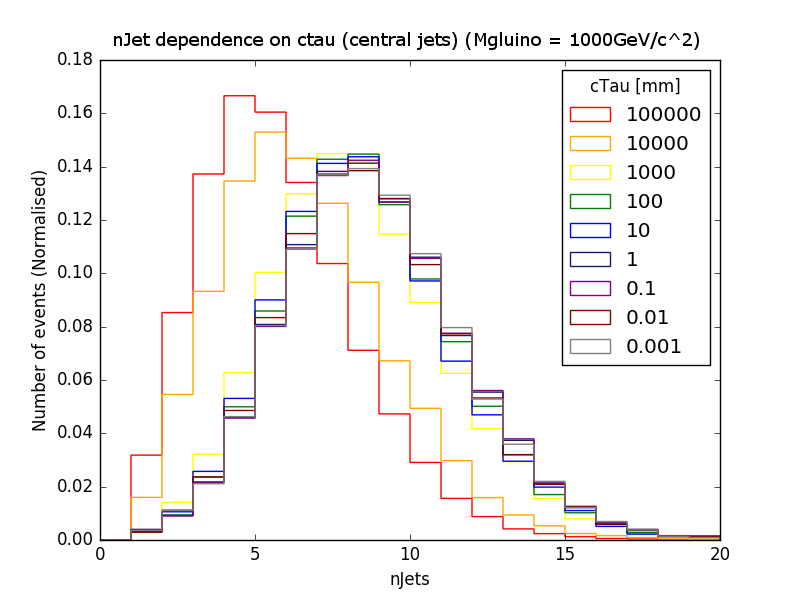
\includegraphics[width=9cm]{ctaunjetclean.png}
\caption{Dependence of the distribution of central jets on $c_{\tau}$.}
	\label{njet2}	
\end{figure}

For forward jets only, the peaks of both distributions have shifted towards having a larger number of jets, with the same $c_{\tau}$ split as seen in the central jets, peaking at 6.1 and 11.0. 

\begin{figure}[H]
\centering
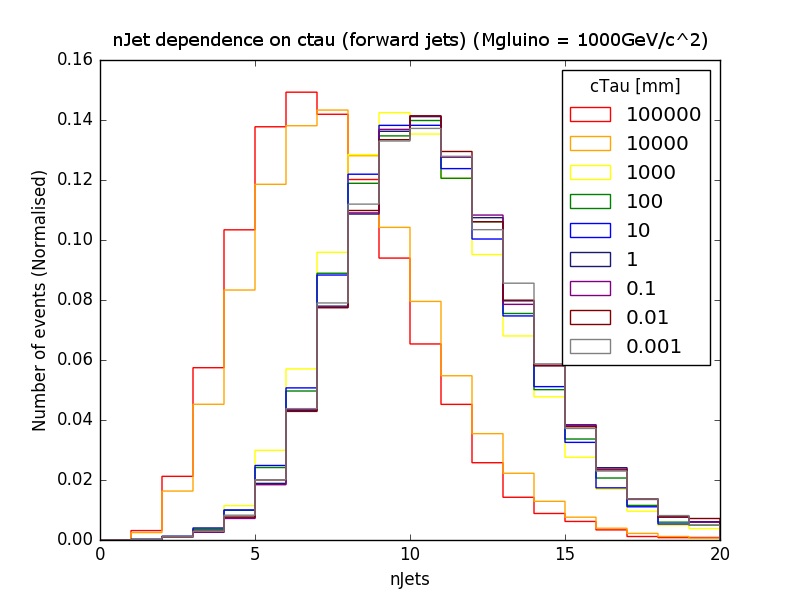
\includegraphics[width=9cm]{ctaunjetfor.png}
\caption{Dependence of the distribution of forward jets on $c_{\tau}$.}
\end{figure}

Combining these two regions in Figure \ref{njet4}, the average number of high-lifetime jets becomes 10.0 and the average of the ISR jets becomes 5.7. 

\begin{figure}[H]
\centering
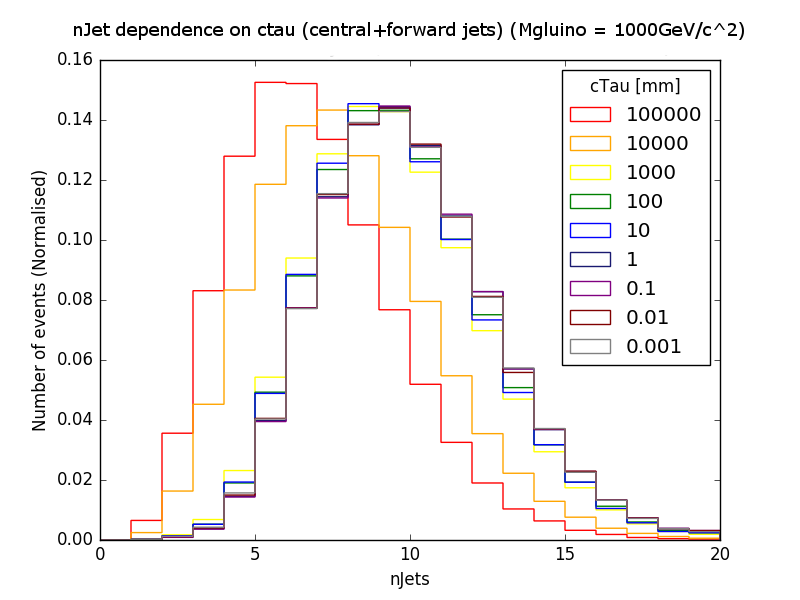
\includegraphics[width=9cm]{ctaunjetfc.png}
\caption{Dependence of number of jets on $c_{\tau}$ for both forward and central jets.}
	\label{njet4}
\end{figure}

Comparing the number of jets per event for different LLP masses in Figure \ref{njet5}, there is a small change in shape, but the dependencies seem to be small, since the mean number of jets in both cases remains the same. This would be expected since in both cases, the physics is the same regardless of the mass of the gluinos, which will always decay into the same number of jets.

\begin{figure}[H]
\centering
\includegraphics[width=16cm]{ctaunjetcomp.png}
\caption{Comparison of the distributions for different LLP masses.}
	\label{njet5}
\end{figure}

\subsection*{Effectiveness of JetId and cut efficiencies}

JetId is a series of cuts designed to eliminate background as much as possible from a sample. There are two strengths, which vary in the fraction of neutral hadrons and neutral EM particles they allow in events with the jets, with other cuts being made on the number of constituents and charged hadron and EM fractions. There is also a cut on the charged multiplicity, which is not considered in this analysis since the data information did not include it.  

Figure \ref{id1} shows the difference in Ht distribution at $c_{\tau}$ = 1mm for all the gluino masses with and without the JetId cuts. There is a slight difference in the shape, particularly for the lower masses, but overall there is not large difference between the two. 

\begin{figure}[H]
\centering
\includegraphics[width=16cm]{htidcomp.png}
\caption{Comparison of the Ht dependence on the LLP mass at pT$>$30 GeV/c and $\eta < $2.4 at $c_{\tau}$ = 1mm.}
	\label{id1}
\end{figure}

In order to numerically quantify the difference the JetId makes, the number of jets with and without JetId was counted and plotted for different $c_{\tau}$ values. Before applying the Id, the usual pT, $\eta$ and number of jet cuts were made. As shown in Figure \ref{id2} and the table \ref{idt1}, for short lifetimes there is a very small difference made by the Id, but it is barely noticeable, with a change of approximately 0.006$\%$ in the number of jets. For longer lifetimes, the change is slightly larger, but still only removes 3.1$\%$ of the jets at most when $c_{\tau}$ = 1000mm. 

\begin{figure}[H]
\centering
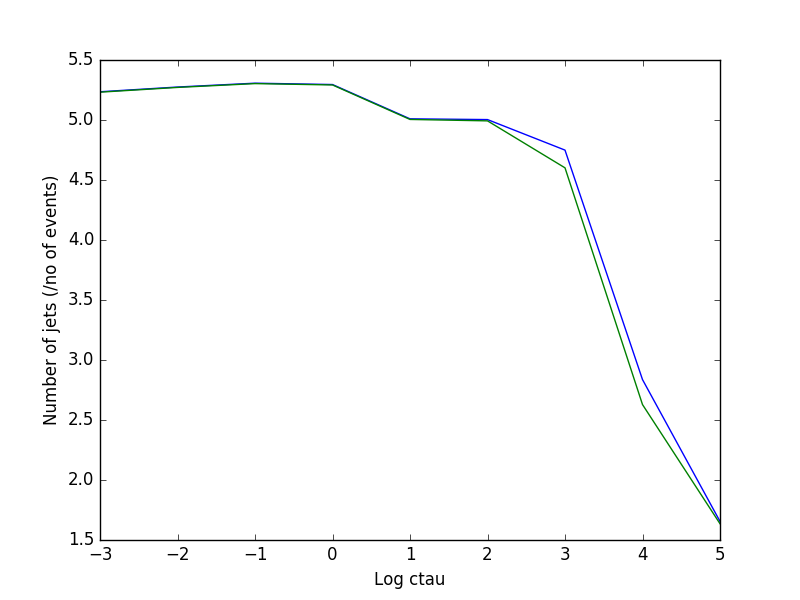
\includegraphics[width=9cm]{RNjetidcomparison.png}
\caption{Number of jets /number of events with and without JetId, in order to determine how much of a difference it makes. At low  $c_{\tau}$, very few jets are being excluded by it, and even at high  $c_{\tau}$ the effect remains small.}
	\label{id2}
\end{figure}

\begin{table}
\begin{center}
\begin{tabular}{ |c|c|c|c|c|c|c|c|c|c| } 
 \hline
 c$\tau$ &0.001 & 0.01 & 0.1 & 1 & 10 & 100 & 1000 & 10000 & 100000 \\ 
 \hline

Without JetId & 5.235& 5.275& 5.307& 5.296& 5.010&
 5.004& 4.749& 2.837& 1.655\\
 \hline
With JetId & 5.232& 5.272& 5.303& 5.292& 5.005& 4.993&
 4.601& 2.629& 1.636 \\
 \hline

\end{tabular}

\caption{Table of numerical values from Figure 8.}
	\label{idt1}
\end{center}
\end{table}

To investigate this effect, the individual efficiencies of the cuts within the JetId were calculated and plotted for different lifetimes, with the exception of the number of constituents since in this case that cut had no effect. The efficiencies of only considering central jets and a harsher pT cut were also considered. These were applied cumulatively, to estimate the best possible theoretical efficiency which could be achieved, since experimental errors would lower the efficiency further.

\begin{figure}[H]
\centering
\includegraphics[width=9cm]{effncutRN.png}
\caption{Cutflow plot of the pT, eta and loose JetId cuts, applied cumulatively.}
\end{figure}

The largest effect is the pT cut, followed by the charged hadron fraction and neutral hadron fraction, though the effects of the JetId cuts are only significant for longer lifetimes. Numerical values can be seen in table \ref{idt2}. 

\begin{table}
\begin{center}
\begin{tabular}{ |c|c|c|c|c|c|c|c|c|c| } 
 \hline
 c$\tau$ &0.001 & 0.01 & 0.1 & 1 & 10 & 100 & 1000 & 10000 & 100000 \\ 
 \hline

 pT$>$150GeV & 0.660& 0.662& 0.662& 0.662& 0.655& 0.653& 0.639& 0.551& 0.461\\
 \hline
 $\eta<2.4$ & 0.619& 0.621& 0.621& 0.621& 0.612& 0.609& 0.593& 0.492& 0.380 \\
 \hline
 chf$>$0 &0.618& 0.621& 0.621& 0.621& 0.612& 0.608& 0.580& 0.479& 0.379 \\
 \hline
 cemf$<$0.99 & 0.618& 0.621& 0.621& 0.621& 0.612& 0.608& 0.580& 0.479& 0.379\\
 \hline
 nhf$<$0.9 & 0.618& 0.621& 0.621& 0.620& 0.612& 0.608& 0.568& 0.432& 0.372 \\
 \hline
 nemf $<$0.9& 0.617& 0.620& 0.620& 0.619& 0.610& 0.607&
 0.566& 0.430& 0.371\\
 \hline
\end{tabular}

\caption{Table of numerical efficiency values from Figure 9. }
	\label{idt2}
\end{center}
\end{table}

To look more closely at the JetId cuts themselves, the plot was renormalised to consider only jets satisfying the pT and $\eta$ cuts for both tight and loose Id. These can be seen in Figures \ref{id3} and \ref{id4}. 

\begin{figure}[H]
\centering
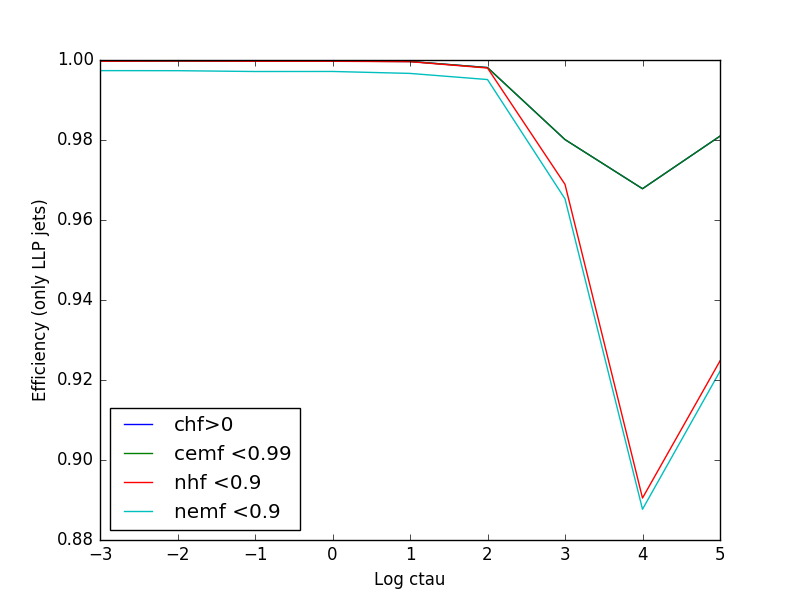
\includegraphics[width=9cm]{effncutrnlltight.png}
\caption{Efficiencies of just the tight JetId cuts, after renormalisation to the pT and eta cuts. The efficiency remains close to 1 until the gluinos start decaying outside the detector, and then drops steeply.}
	\label{id3}
\end{figure}

\begin{figure}[H]
\centering
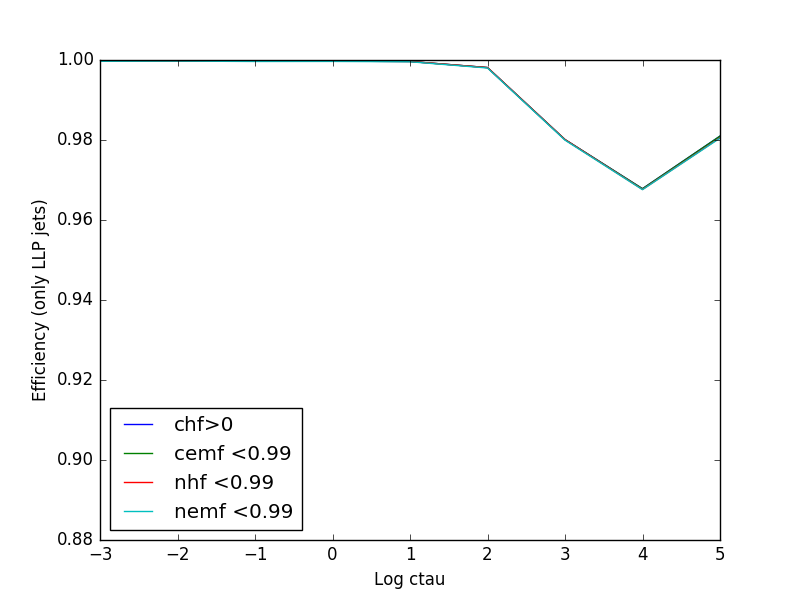
\includegraphics[width=9cm]{effncutrnllpl.png}
\caption{Figure 10 replotted, but for loose JetId. Here, the NHF and NEMF make very little difference to the efficiency, with CHF being the main variable causing a drop.}
	\label{id4}
\end{figure}

\begin{table}
\begin{center}
\begin{tabular}{ |c|c|c|c|c|c|c|c|c|c| } 
 \hline
 c$\tau$ &0.001 & 0.01 & 0.1 & 1 & 10 & 100 & 1000 & 10000 & 100000 \\ 
 \hline

 nhf$<$0.99 &0.618& 0.621& 0.621& 0.621& 0.612& 0.608& 0.580& 0.478& 0.379\\
 \hline
 nemf $<$0.99& 0.617& 0.621& 0.621& 0.620& 0.612& 0.607& 0.579& 0.477& 0.379\\
 \hline
\end{tabular}

\caption{Efficiencies for the neutral hadron fraction and neutral EM fraction cuts in the tight JetId limits, after applying the pT, eta chf and cemf cuts as in the previous table.}
\end{center}
\end{table}

In both of these, there is very little change in efficiency until longer lifetimes are reached, implying that the both the gluino and ISR jets are quite tightly limited in all the variables in question by the physics already. Thus, there is unlikely to be a need to refine the JetId cuts further for greater efficiency. 

A feature to note in the above plots is that despite a steep decrease in efficiency for longer $c_{\tau}$, the final efficiency seems to increase. This is likely to be due to statistics rather than any underlying physics, since the number of LLP jets drops extremely steeply, so there is not a large enough sample size at the final lifetime to calculate the efficiency accurately as shown in Figure \ref{id5}.

\begin{figure}[H]
\centering
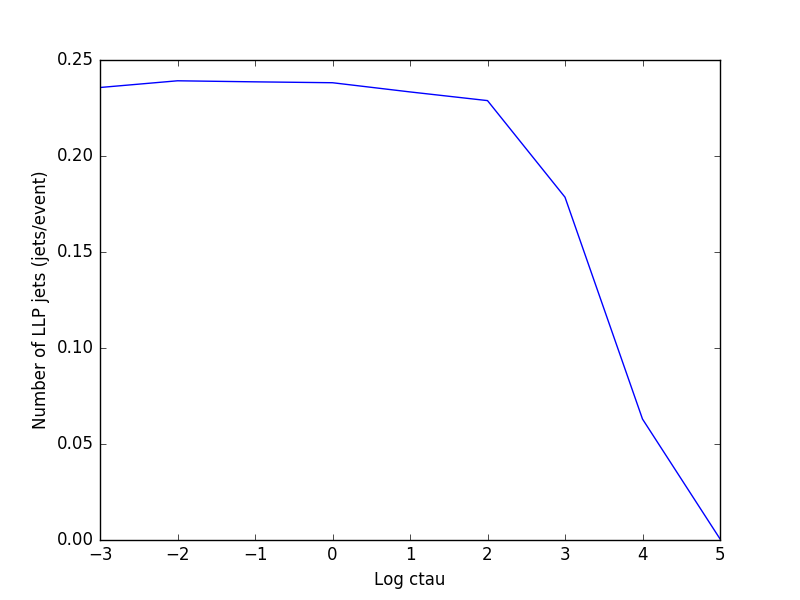
\includegraphics[width=9cm]{RNeffllpnumber.png}
\caption{How the number of jets from gluinos varies with $c_{\tau}$. The actual number of jets drops to 117, compared to 572800 at $c_{\tau}$ = 0.001.}
	\label{id5}
\end{figure}

\subsection*{Analysis of gluino jets and invariant mass}
In previous sections, if the gluino jets needed to be specifically targeted, a genlevel boolean variable was used to select them. However, when analysing real data, this is not possible, so other methods of identifying the gluino jets need to be developed. 

One way to do this is to use the invariant mass, which if it is non-zero gives an estimate for the gluino mass, as well as aiding identification of the jets and separation from the ISR. Initially, the gluino jets were chosen as the four jets which when paired off gave the two highest invariant masses, and the dependence of this on $c_{\tau}$ plotted in Figure \ref{im1}.

Then, to check the selection method, the invariant masses of the two pairs were plotted against each other in a scatter plot. This was done to check whether the two masses were similar, since it would be expected that the gluinos would be produced with the same mass. The resultant plot does appear to verify this, with a larger spread than expected, so for later plots the gluino jets were chosen as the pairs with the most similar invariant mass. This, however, still only changed the jets chosen in 10.1$\%$ of cases, so the previous method continued to be used. The slight bias of Figure \ref{i2} towards the x-axis is due to the order of the jets stored in the event trees, rather than any underlying physics. Due to jets being stored in decreasing pT order, when making the selection of the two highest invariant mass jets, the first jet selected is more likely to have the higher mass, explaining the skew. If jets are assigned to x and y randomly, the spread becomes symmetrical around the line y=x as expected. 


\begin{figure}[H]
\centering
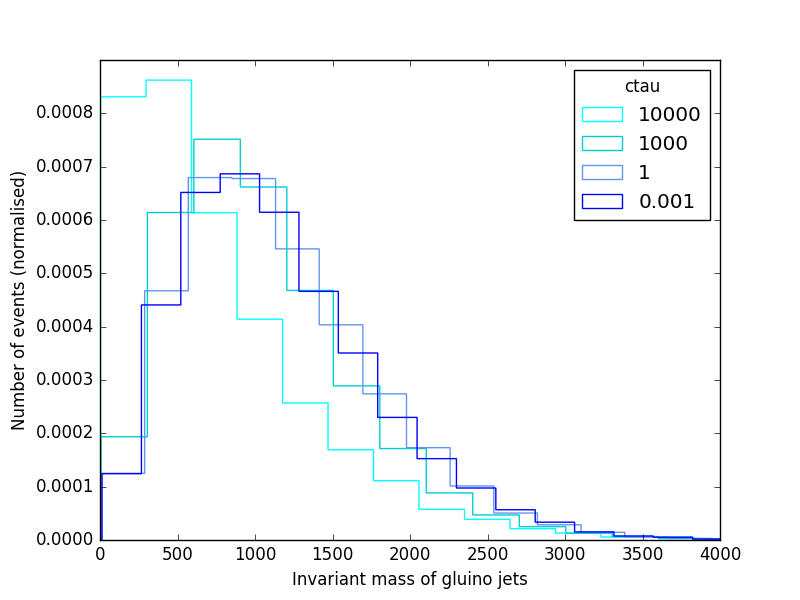
\includegraphics[width=9cm]{imassgjetctau.png}
\caption{FIX THIS LABEL IS WRONG! Dependence of the invariant mass on $c_{\tau}$.}
	\label{im1}
\end{figure}

\begin{figure}[H]
\centering
\includegraphics[width=9cm]{mjetcomparisonnonrandom.png}
\caption{Scatter plot of the invariant masses of the two gluino jets, selected by highest mass pairs.}
	\label{i2}
\end{figure}

It would be expected that the invariant mass of the jets has a strong correlation with the gluino mass, so Figure \ref{im3} was plotted to verify this. Indeed, the mass distribution peaks near to the LLP mass of that particular sample, though at low masses this becomes less reliable. This provides a reasonable way to estimate the mass of the gluino. The mass asymmetry of the jets was also investigated and found to be non-zero for longer lifetimes, which would be expected because (???). 



\begin{figure}[H]
\centering
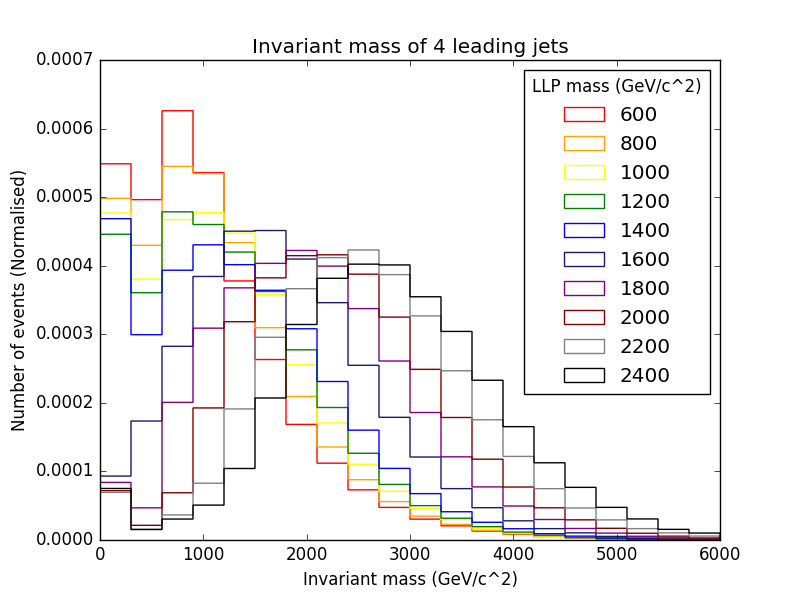
\includegraphics[width=9cm]{imassllp.png}
\caption{Dependence of the invariant mass of the gluino jet pair on the LLP mass. THIS IS FOR PAIRS OF JETS MAKE IT CLEARER SOMEHOW.}
	\label{im3}
\end{figure}

\begin{figure}[H]
\centering
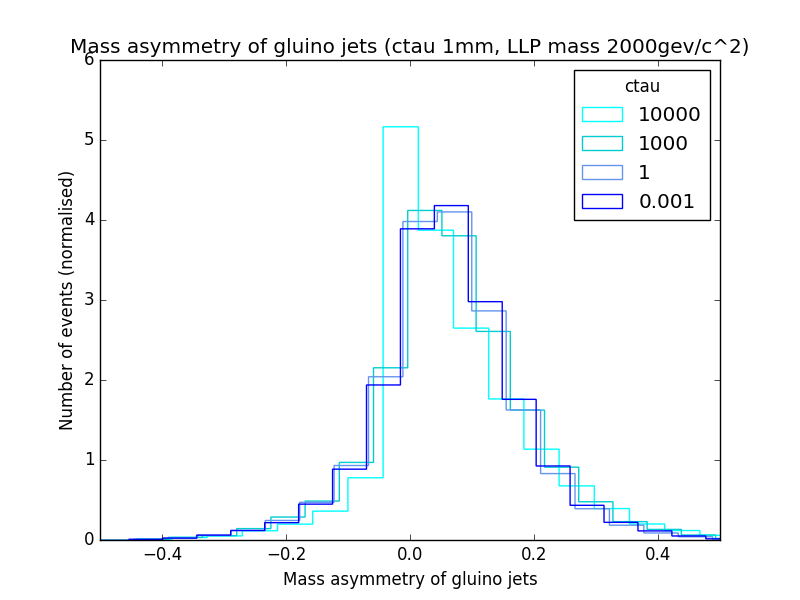
\includegraphics[width=9cm]{massasymctau.png}
\end{figure}

With the gluino jets suitably identified and checked, the transverse momentum of all the jets and the missing energy was added vectorially. This would be expected to be zero if all the constituents were included, however due to the presence of the LSP particle, the vector sum will be non-zero, have magnitude equal to the LSP and point in the opposite direction to the LSP particle's path. The magnitude of the resultant pT can be seen in Figure \ref{im4}, which peaks at 500 GeV/c. 

\begin{figure}[H]
\centering
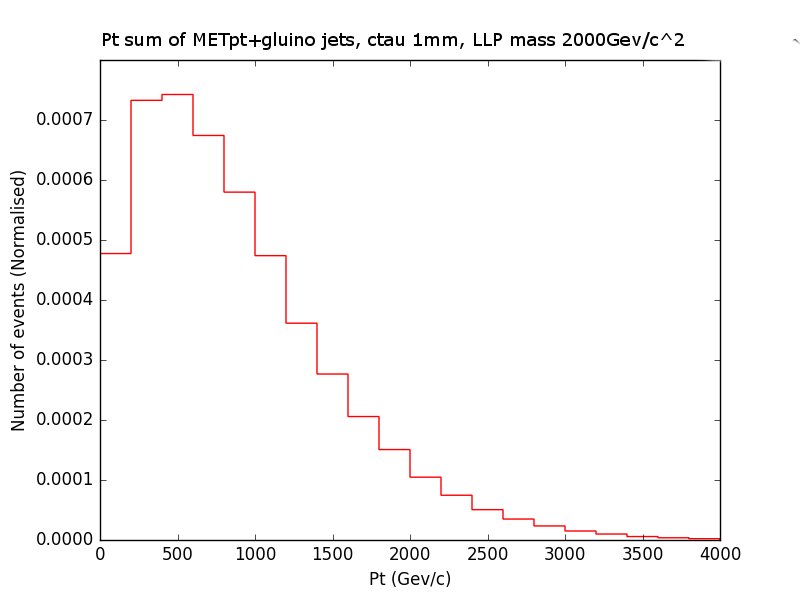
\includegraphics[width=9cm]{lsppt.png}
\caption{The pT sum of all 4 gluino jets and the missing energy.}
	\label{im4}
\end{figure}

The difference in eta between the gluino jets was also plotted, and as Figure \ref{im5} shows the eta difference peaks at zero, implying that the jets are most commonly formed in the same transverse plane. This is useful when reconstructing the LSP properties as done above.

\begin{figure}[H]
\centering
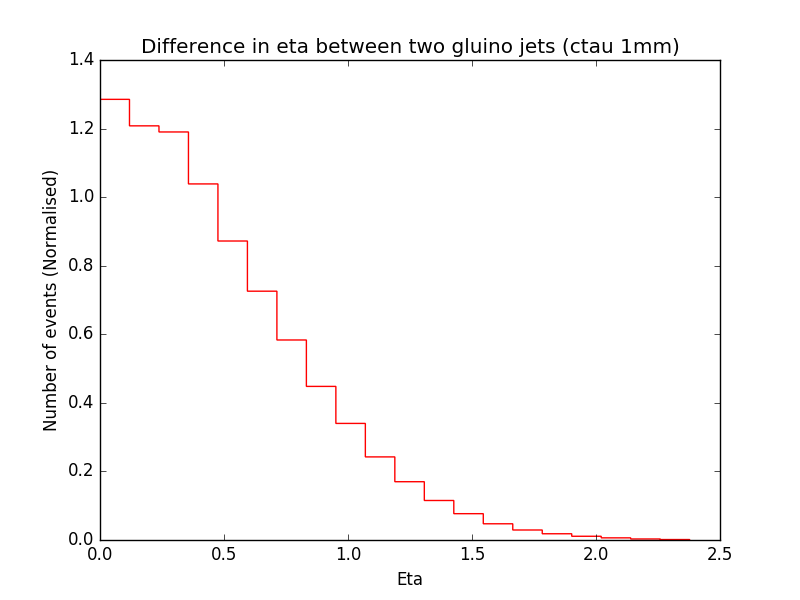
\includegraphics[width=9cm]{etadiffglu.png}
\caption{The magnitude of the difference in $\eta$ between the two gluino jet pairs.}
	\label{im5}
\end{figure}

\subsection*{Compressed and uncompressed cases}
The aim here was to determine whether the two cases were significantly different for any variables with a strong dependence on the gluino mass. Here, the compressed case is defined as $M_{LLP}$ = 1000 GeV/$c^{2}$ and $M_{LSP}$ = 900 GeV/$c^{2}$, and the uncompressed case as $M_{LLP}$ = 1800 GeV/$c^{2}$ and $M_{LSP}$ = 200 GeV/$c^{2}$.

Firstly, the invariant mass of the gluino jets was considered. As Figure \ref{c1} shows, these two distributions are very well separated, so the combination with the strong gluino mass dependence makes this an excellent variable to use for analyses. Similarly, the Ht of the jets is also well separated, as shown in Figure \ref{c2}, though the dependence on LLP mass is less strong. 

\begin{figure}[H]
\centering
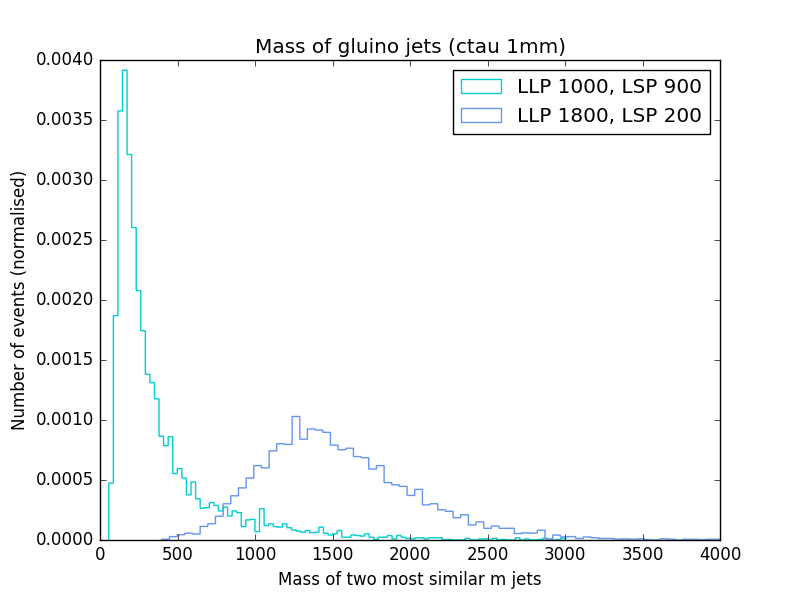
\includegraphics[width=9cm]{imasscompboth.png}
\caption{Comparison of invariant mass distributions for compressed and uncompressed cases.}
	\label{c1}
\end{figure}

\begin{figure}[H]
\centering
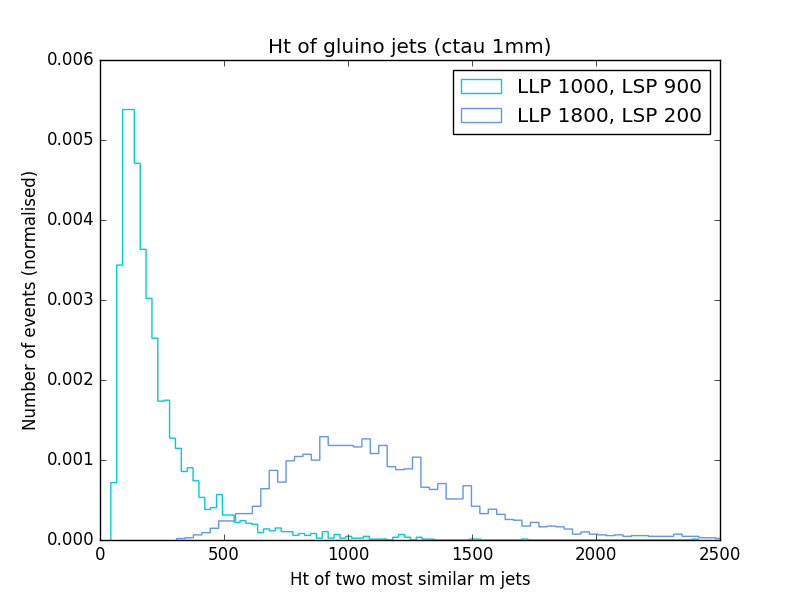
\includegraphics[width=9cm]{htcompboth.png}
\caption{Comparison of Ht distributions for compressed and uncompressed cases.}
	\label{c2}
\end{figure}

The mass asymmetry was also considered, however the two cases overlap heavily, with the only key distinction between them being that the compressed case has a much larger fraction of asymmetry near zero. Finally, the average mass of a jet was plotted, which also has distinct shapes and peak positions for the two cases. 

\begin{figure}[H]
\centering
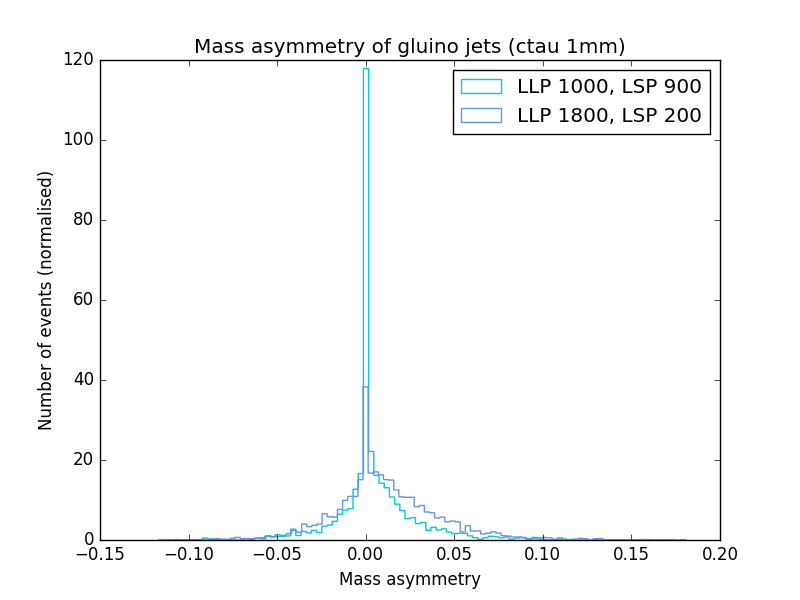
\includegraphics[width=9cm]{astmcompboth.png}
\end{figure}

\begin{figure}[H]
\centering
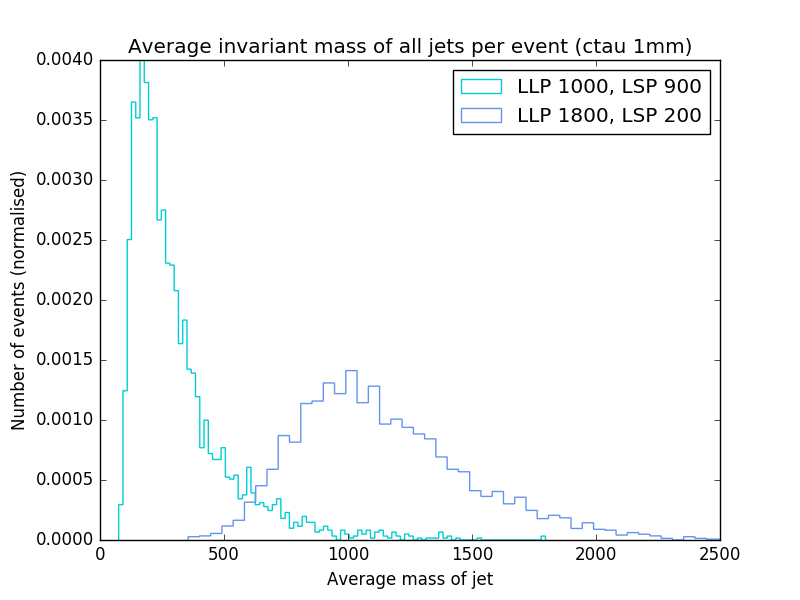
\includegraphics[width=9cm]{avmasscentjets.png}
\end{figure}

\section*{Conclusions}
heh lol idk




%\begin{figure}[H]
%\centering
%\includegraphics[width=16cm]{effncut.png}
%\end{figure}

\end{document}
